\chapter{Design and Implementation} \label{chap:impl}

<<<<<<< HEAD
=======
%FOCUS ON BIOLOGISTS/USABILITY

>>>>>>> d36f4c58ce53756c4208d542755ca45e64177c23
The primary deliverable of this dissertation is a system, \gls{sys} (shown in Figure \ref{fig:overview}) that is able to generate metabolic models of cell-free systems.
This chapter decomposes \gls{sys} into its four main parts.
First, \gls{sys} ingests experimental data and converts it into a standardized format.
Next, \gls{sys} uses the data to construct a group of cellular metabolic models and sample fluxes from those models to create a dataset.
Then, \gls{sys} performs dimensionality reduction to elucidate underlying trends in the experimental data.
Finally, \gls{sys} leverages those insights to reduce the original, overspecified models to standalone cell-free metabolic models.

\section{Data gathering}
In order to build a robust model that reflects biological reality, I first had to generate data to use for training.
Gathering high quality biological data is difficult and is crucial to the success of the system as a whole.
I describe the high level process of creating a cell-free system and running the experiments below.
The full experimental protocol can be found at dx.doi.org/10.17504/protocols.io.kz2cx8e.

\begin{figure}[t!]
\begin{center}
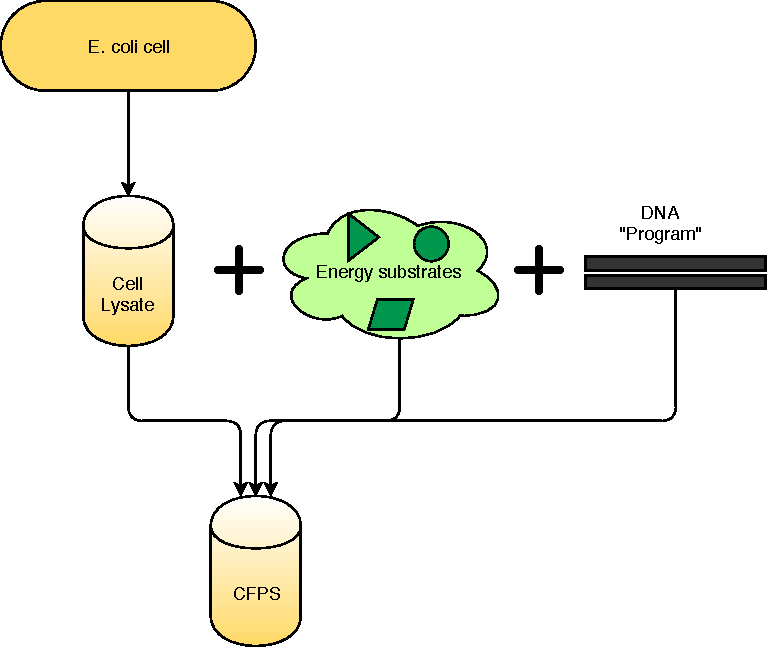
\includegraphics{figs/CellFreeSetup.pdf}
\caption[Process for creating a \gls{cfps} system]{Process for creating a \gls{cfps} system.
The \gls{ecoli} cells can be grown up in bulk, allowing future preparation of \gls{cfps} reactions to be far quicker than typical \textit{in vivo} methods.
}
\end{center}
\label{fig:cfps}
\end{figure}

\subsection{Cell-free systems}
As shown in Figure \ref{fig:cfps}, creating a cell-free protein expression system involves three main steps: growing and lysing cells, supplementing with energy substrates, and adding custom \gls{dna} constructs.
This protocol is based on an open protocol from the Federici lab \cite{medina2017cfps}.
I began by growing up 1L of BL21 \gls{ecoli} cells in an overnight culture of \gls{lb} until they reached an \gls{od} of 1.6.
The cells were then split into 45 \gls{ml} aliquots centrifuged for 12 minutes at 4500\textit{g}~and the supernatant is poured off.
The pellet was then be stored in a 4\degree~refrigerator overnight if necessary.
Next, the cells underwent 2 more sets of centrifugation with the same settings; the pellet was resuspended each time with 45 \gls{ml} of S30A buffer (see Appendix \ref{app:exp} for buffer compositions).
The cells were then centrifuged twice more at 2000\textit{g}~ for 8 and 2 minutes.
In between the final two centrifugations, the cells were resuspended with 37.5 \gls{ml} of S30B buffer.
After the final centrifugation step, the pellets were weighed and resuspended with $0.9$ times their weight in S30A and $5$ times their weight of $0.1$ mm beads.
Using a bead beater set to 46 rpm, the cells were beaten for 30 seconds, rested on ice for 1 minute, and then beaten for another 30 seconds.
These lysed cells were spun one final time for 8 minutes at 4500\textit{g}~to remove the cellular debris and beads.
The supernatant was then removed as a cell extract and stored in a -80\degree~freezer.

This cell extract contains the core cellular machinery that is necessary for transcription and translation.
However, the full \gls{cfps} system requires additional reactants that are important for the transcription and translation reactions.
The addition of these reactants to the cell extract creates a full \gls{cfps} system.
These substrates include cofactors such as \gls{camp}, maltodextrin, and \gls{nad}, as well as vital building blocks of transcription and translation such as \glspl{ntp}, \glspl{aa}, and \glspl{trna}.
Table \ref{tab:cf-nrg} lists each of the reactants and their purpose in the cell-free system, while Table \ref{tab:cf-conc} shows the final concentration for each reactant.

This cell-free expression system acts a biological computer.
Whatever \gls{dna} ``program" is added, the system will work to produce the appropriate protein result.
This platform is powerful because it allows a user to easily insert these \gls{dna} programs and see results within a few hours.
A typical biological timeline would take far longer because living cells would have to be transformed (a lengthy process) to uptake the \gls{dna} and incorporate it into their production processes.

\begin{table}[]
\centering
\begin{tabular}{lll}
\textbf{Reactant }    & \textbf{Amount} (\gls{ul}) & \textbf{Purpose}                        \\
Maltodextrin solution          & 5               & Energy substrates               \\
Amino acids         & 10              & Building blocks for \gls{tl} \\
\gls{peg}          & 2.5             & Molecular crowding              \\
\gls{hmp}          & 1               & Phosphate source                \\
\gls{mg}           & 0.74            & Important cofactor              \\
\gls{k}            & 0.8             & Charge homeostasis              \\
\gls{dna}          & 0.8             & Template for protein   \\
Cell extract & 25              & \gls{tx}/\gls{tl} machinery                 \\ \hline
\gls{cfps} system        & 50              & Protein production             
\end{tabular}
\caption[List of reactants for a 50 \gls{ul} \gls{cfps} reaction]{List of reactants for a 50 \gls{ul} \gls{cfps} reaction. 
See the final concentrations of all reactants in Table \ref{tab:cf-conc}.
Note that MDX is a mixture of substrates (also detailed in Table \ref{tab:cf-conc}).
Amino acids includes all 20 of the amino acids.
}
\label{tab:cf-nrg}
\end{table}

\begin{table}[]
\centering
\begin{tabular}{llll | l}
Sugar & \gls{hmp} & \Glspl{ntp} & \gls{k} & Normalized output   \\ \hline
0    & 0    & 1    & 0    & 0.57 \\
0    & 1    & 0    & 0    & 0.52 \\
1    & 0    & 0    & 0    & 0.59 \\
0    & 0.5  & 0.5  & 0    & 0.97 \\
0.5  & 0    & 0.5  & 0    & 0.76 \\
0.5  & 0.5  & 0    & 0    & 0.20 \\
0.25 & 0.25 & 0.5  & 0    & 0.40 \\
0.25 & 0.5  & 0.25 & 0    & 1.00 \\
0.5  & 0.25 & 0.25 & 0    & 0.96 \\
0.25 & 0.25 & 0.25 & 0.25 & 0.36 \\
0    & 0    & 0    & 1    & 0.19 \\
0    & 0    & 0.5  & 0.5  & 0.22 \\
0    & 0.5  & 0    & 0.5  & 0.16 \\
0.5  & 0    & 0    & 0.5  & 0.16 \\
0    & 0.25 & 0.25 & 0.5  & 0.37 \\
0.25 & 0    & 0.25 & 0.5  & 0.47 \\
0    & 0.5  & 0.25 & 0.25 & 0.26
\end{tabular}
\caption[Different reaction concentrations for our Manual dataset]{Different reaction concentrations for our Manual dataset.
Reactant columns are measured in \gls{ul}, while the output column has been normalized by the maximum level of fluorescence observed.
Each experiment was repeated $n = 2$ times at a total volume of 6\gls{ul}.
}
\label{tab:manual}
\end{table}

\subsection{Datasets}
The protocol above was used to create two datasets for training.
The first dataset was created by hand and followed standard lab procedures.
Each of the reactants specified by Table \ref{tab:cf-nrg} was combined in the appropriate ratio to create a 200 \gls{ul} mastermix. 
That mastermix was then split into 5 \gls{ul} aliquots.
1 \gls{ul} of varying concentrations of the energetic substrates were added to each aliquot, bringing the total reaction volume to 6 \gls{ul} .
This dataset is composed of 17 differing ratios of sugar, phosphate, potassium, and nucleotides.
I used a \gls{dna} circuit that encodes the \gls{rfp} gene, so the amount of protein production was measured using fluorescence readout with a plate reader.
The results for those reactions are shown in Table \ref{tab:manual}

One of the downsides to generating this data by hand is that creating large datasets by hand takes a long time.
To increase the amount of data generated, I created a second dataset using a Labcyte Echo acoustic liquid handler.
The Echo is an acoustic liquid handler that can programmed to combine different amounts of liquid.
Using the Echo, I was able to generate a larger number of different experimental conditions for the \gls{cfps} reactions.
Additionally, pipetting by hand has intrinsic error, while the Echo is able to transfer liquids in multiples of 2.5 \gls{nl} with less than 2\% error.
The Echo therefore has the dual benefits of generating more data and reducing the amount of noise in that data.
The experiments on the Echo were performed using 2\gls{ul} of \gls{cfps} system and 500 \gls{nl} of additional reactants.
The use of automation allowed us to test 51 different reaction conditions and shows that this could be expanded to an even larger scale.

Finally, I also used a third dataset from the recent Karim and Jewett paper that uses \gls{cfps} systems to perform metabolic engineering~\cite{karim2018controlling}.
Their protocol is very similar to the one I showed above, though the final composition of the reactants differs.
This dataset is useful because it was created in a different lab and they measured the output using liquid chromatography, not fluorescence.
Since this dataset was created in different lab conditions, it can be used to check that our system is generalizable to cell-free systems as a whole and not just overfitting data generated from my \gls{cfps} system.

We will refer to these datasets as our "Manual", "Echo", and "Karim" datasets.

\begin{figure}[t!]
\begin{center}
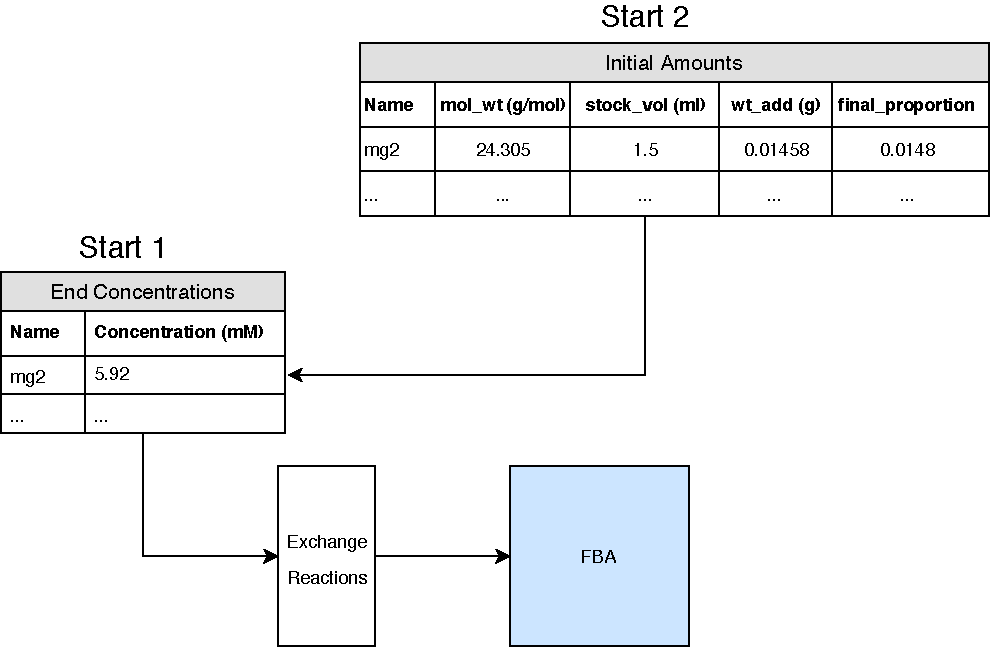
\includegraphics[width=\textwidth]{figs/DataIngestion.pdf}
\caption[Data ingestion part of \gls{sys}]{Two possible ways to incorporate the experimental setup in \gls{sys}.
In Start 1, the user already knows the final concentrations of each reactant and can upload that as a \gls{csv}.
Otherwise, the user can upload information about the reactants that are added and our tools will automatically calculate the final concnetrations of each reactant.}
\label{fig:ingest}
\end{center}
\end{figure}

\section{Data ingestion and incorporation}

\subsection{Data ingestion}
Since this system is intended to aid biologists in their experiments, I designed it to be usable without any coding experience.
With that in mind, I created two separate ways to incorporate the experimental setup into the models.
Figure \ref{fig:ingest} shows the acceptable structures of the experimental setup .
The first structure is a \gls{csv} containing the final concentrations of the different reactants in the cell-free system.
This is the easiest to incorporate because it is a simple conversion from concentrations to fluxes.
Fluxes have the unit mol/min/gDW, so they can be converted from metabolite concentrations into fluxes using the following equation from MetaboTools~\cite{aurich2016metabotools}:
\begin{equation}
f = \frac{m}{c * t * 1000.0}
\end{equation}
where $f$ is the flux value, $m$ is the concentration of our metabolite, and $c$ is the overall concentration of the cell.
I used $t = 24$ because our reactions ran for 24 hours.
Using this equation, \gls{sys} is able to ingest a \gls{csv} mapping the name of the reactant to the final concentration and turn them into flux constraints.

However, \gls{sys} also supports users who might only know the relative amounts of each reactant that they are adding, but not the final concentrations of their reactants.
This is important because many biologists may have a protocol that they follow that tells them how to make a \gls{cfps} system, but they may not know the final concentrations in their mixture.
\gls{sys} allows those users to use a \gls{csv} (or combination of \glspl{csv}) that contains information about each reactant used to make the system.
Each row has the name of the reactant, its molecular weight, the weight used to create the stock, the volume used to create the stock, and the final volume of the stock added to the cell-free reaction.
Using this information, \gls{sys} calculates the final concentration of each reactant in the \gls{cfps} system and converts it to the same form as the other branch of the pipeline.
Once the data is in its canonical form of final concentrations, \gls{sys} proceeds with the a unified computational pipeline.

\subsection{Data Incorporation} \label{sec:incorp}
After ingesting the experimental setup, \gls{sys} incorporates it into a \gls{fba} model.
The \gls{fba} models are handled via the \gls{cobra}py python package~\cite{ebrahim2013cobrapy}.
\gls{sys} uses the iJO1366 model for its base model of \gls{ecoli}.
iJO1366 consists of 1805 metabolites and 2583 reactions~\cite{orth2011comprehensive}.
This model describes \gls{ecoli} cells, and needs to be adapted to cell-free systems because they no longer have the same physical structure as \gls{ecoli} cells.
First, \gls{sys} changes every reaction reflect the fact that there are no longer any membranes or cellular compartments.
Every reaction that contains a periplasmic or extracellular component is moved into the cytosol.
This is handled by replacing every metabolite in the model with its corresponding cytosolic version.
If no corresponding cytosolic metabolite exists, \gls{sys} creates a cytosolic version of the metabolic and then proceeds as above.
After this step, all of the reactions in the model occurring in the same compartment, which reflects how a \gls{cfps} system works.

\gls{sys} then handles the specific experimental data that was earlier ingested through the use of exchange reactions.
Exchange reactions are pseudo-reactions that allow a \gls{fba} model to constrain the amount of a reactant present in the model.
For each of the reactants in a \gls{cfps} system, \gls{sys} creates an exchange reactions with bounds based on the fluxes that were calculated earlier.
At the end of this process, \gls{sys} has converted the full-scale \gls{ecoli} model to better approximate a \gls{cfps} system.
This type of model has not been generated before, but it is still overspecified.
This model is what is later used to reduce into a base cell-free model.

\gls{sys} also provides the option to explicitly incorporate the transcription and translation reactions that are so crucial to \gls{cfps} systems.
Most \gls{fba} models do not explicitly model the transcription and translation reactions.
However, earlier work from the Varner lab incorporated these reactions into a \gls{fba} model specifically to try to model a cell-free system~\cite{vilkhovoy2017sequence}.
This earlier work created the \gls{fba} model by hand and is written in Julia.
\gls{sys} provides auxiliary tools to, given the sequence of the gene of interest, automatically generate a relevant version of the Varner model.
That model is converted to Python and the relevant transcription and translation reactions are extracted.
Those reactions are then incorporated into the base cell-free model, creating a TXTL cell-free model.
<<<<<<< HEAD
=======

%As a linear programming problem, we also need to set a custom objective to optimize for.
%Usually this is the biomass objective, which encapsulates everything necessary for bacterial growth.
%However, since we don't care about growth, just production, we can use our own objectives.
%For us, the typical objective will be the production of some protein since that's the purpose of the \gls{cfps}.
>>>>>>> d36f4c58ce53756c4208d542755ca45e64177c23

\section{Dataset generation}

\subsection{Model generation}
Once \gls{sys} has created these base models, it uses them to create a different model for each experimental condition.
\gls{sys} reads in a \gls{csv} consisting of the experimental conditions and a quantitative output.
Each row represents a different experiment and each column contains the amount of additional reactant that was added.
\gls{sys} then re-calculates the final concentrations of each of the reactants for each experimental starting condition.
Those new concentrations are used to update the constraints for the exchange reactions of each reactant.
For each unique experimental condition, \gls{sys} creates a new \gls{fba} model.

These experimental condition models are still overspecified and therefore have the same optimal solution.
Thus, these naive models poorly describe the biological reality of the datasets (see Section \ref{sec:cmp} for a comparison).
Clearly, \gls{fba} does not describe what is occurring in a \gls{cfps} system.
These \gls{fba} models contain every reaction that is occurring in a steady state bacterium.
While the bacteria are harvested at steady state, not all reactions will maintain their importance in a cell-free system.
I hypothesized that these base models failed to describe cell-free systems because the differences between a cell-based system and a cell-free system cannot be encapsulated solely through different exchange reactions and the creation of a single-compartment system.

\gls{fba} acts as a coarse, non-linear amplifier, so points that vary only slightly in the input parameter space may not differ very much in the output space.
I wanted to improve the granularity of \gls{fba} response by passing the fluxes through a dimensionality reduction technique such as a \gls{vae}.
In order to do this, I needed a large dataset of fluxes to train on.
Although the experimental conditions led to only have a small number of models, I was able to create large datasets by flux sampling from each model.

\begin{figure}[t!]
\begin{center}
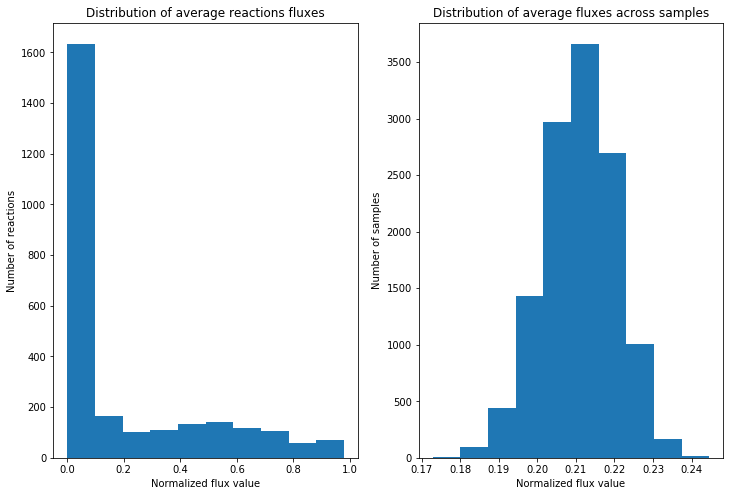
\includegraphics[width=\textwidth]{figs/fluxdistribution.png}
\caption[Distribution of fluxes generated by flux sampling]{Distribution of fluxes generated by flux sampling.
X axes represent the value of the fluxes and have been scaled to between 0 and 1.
The plot on the left shows a histogram of the average flux value for each reaction.
Most reactions have an average flux that is close to 0.
The right plot shows the average flux across samples.
The average flux across all samples clusters around 0.21. 
}
\label{fig:distrib}
\end{center}
\end{figure}

\subsection{Flux sampling}
Flux sampling is the process of sampling possible fluxes through each reaction.
\gls{sys} performs flux sampling on each model of a different experimental condition.
For each model, this generates a distribution of fluxes for every reaction in that model.
Figure \ref{fig:distrib} shows the average distribution of fluxes for each sample and each reaction.
Flux sampling is implemented using the optGpSampler routine~\cite{megchelenbrink2014optgpsampler}.

Each model has different experimental conditions and therefore has slightly different flux distributions for each reaction.
So, after generating flux samples for each model, these sampled fluxes are combined to generate two new datasets.
One dataset is flat---meaning we simply concatenate all of the sampled fluxes into a single dataset.
This dataset has size $(N * E) \times R$ where $N$ is the number of samples, $E$ is the number of experiments, and $R$ is the number of reactions.
This flat dataset is useful to investigate the fluxes using typical dimensionality reduction techniques.
However, \gls{sys} also generates a stacked dataset of size $N \times E \times R$. 
This involves sampling with replacement from the distribution of fluxes of each model and then stacking the fluxes to create a new dataset.
Using this version of the dataset facilitates the training of a Corr-VAE.
I used this part of \gls{sys} to generate flat and stacked versions of all three of the datasets described above.

\section{\gls{vae}} \label{sec:vae}
As mentioned earlier, the base cell-free \gls{fba} models did not describe our experimental data well.
To solve that issue, \gls{sys} implements a \gls{vae} to reduce the dimensionality of our models.
The \gls{vae} is implemented using the Keras framework~\cite{chollet2015keras} and the implementation was designed to be as modular as possible.
Because the Corr-VAE has applications in other parts of biology, I implemented all \glspl{vae} to make it easy to change their parameters.
Thus, my implementation takes in command-line arguments to specify either a flat or stacked dataset, a list of layer sizes, the number of latent dimensions, how to scale the inputs, and whether or not to use the custom correlation loss function.
I also provide sensible default values for those users who have less experience in the field of deep learning.

The structure of the \glspl{vae} we used are as follows.
I experimented with two different layer structures, a 2-layer \gls{vae} with layer sizes 1024 and 256 and a 3-layer \gls{vae} with layer sizes 1024, 1024, and 1024.
The 3-layer \gls{vae} performed much better, so that was the structure I used for all subsequent experiments.
I also tried using latent dimensions of size 2 and 10.
Both 2 and 10 dimensions are able to capture relevant information in their latent space, though future work could use even more latent dimensions.
Activations between layers of both the encoder and the decoder were \glspl{relu}~\cite{nair2010rectified}.
The final layer of the \gls{vae} used a sigmoidal activation to produce scaled fluxes between 0 and 1.

\subsection{Corr-VAE}
Placing a regular \gls{vae} on top of a \gls{fba} model will simply attempt to reconstruct the fluxes.
However, I did not just want to reconstruct fluxes in an unbiased way---I wanted the reconstructed fluxes to correspond to the real-world biological data.
The key insight of a Corr-VAE is that the experimental data can be used to perturb the latent space to better reflect biological reality.
A Corr-VAE incorporates the experimentally determined output values into its loss function.
It does so by adding a loss term consisting of the correlation between the experimental data and the reconstructed flux that represents the objective function.
Recall Equation \ref{eqn:vae-loss} that described the normal \gls{vae} loss function.
The Corr-VAE loss function is now written as:

\begin{equation}\label{eqn:corr-loss}
\mathcal{L}(\theta, \phi) = - E[\log p_{\theta}(x_i | z)] + KL(q_{\phi}(z | x_i) || p(z)) + corr(x_i', d)\\
\end{equation}

where $x_i'$ is the reconstructed data, $d$ is the experimentally determined biological data, and $corr$ is the Pearson correlation between the two.
I also experimented with weighting the correlation loss term to force the representation to be closer to the real world data, but this did not appear to have a large effect.
Corr-VAEs required a stacked dataset in order to calculate the correlation between the experimental data and the output fluxes.
By default \gls{sys} uses a Corr-VAE to reduce the dimensionality of a generated dataset.

\section{\gls{fba} model reduction}
The Corr-VAE is able to generate a lower dimensional representation of the base cell-free models.
\gls{sys} uses the reconstructed representation to create better cell-free models.
After examining the latent space of the Corr-VAE to ensure that it was learning the differences between the models, I was able to use the reconstructed fluxes to reduce the original models.
For each experimental condition model, \gls{sys} uses the reconstructed fluxes from the Corr-VAE to determine which reactions are unimportant.
It does this by creating a threshold and removing any reactions that have a flux under that threshold.
By doing this for each model, it builds up a list of reactions that are not used in any of the experimental models.

\gls{sys} then uses removes all of those reactions from the base model to generate a new cell-free model.
The value of this model is tested by comparing how well the optimal fluxes correlate with the experimental data.
Section \ref{sec:cmp} shows that these reduced models with the differential conditions give us better explanations of experimental data than full \glspl{gem}.
The thresholding is a simple method of identifying which reactions are not important in cell-free systems.
Future work could generate improved reduced models by using more sophisticated reduction techniques in conjunction with the Corr-VAE.